\chapter{Lecture 30 - More Boundary Value Problem Examples}
\label{ch:lec30n}
\section{Objectives}
The objectives of this lecture are to:
\begin{itemize}
\item Illustrate the use of Robin boundary conditions with another example.
\item Show how to solve BVPs with an unknown parameter with \lstinline[style=myMatlab]{bvp5c}.
\end{itemize}
\setcounter{lstannotation}{0}

\section{Example Problem \#1}
\begin{marginfigure}
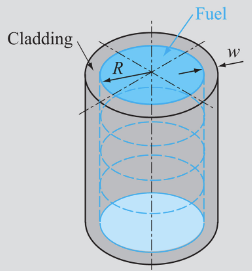
\includegraphics{lec30n-ex1-schematic.png}
\caption{A typical nuclear reactor fuel pin.}
\label{fig:lec30n-ex1-schematic}
\end{marginfigure}
Fuel rods of a nuclear reactor are cylindrical structures with the fuel retained inside cladding material, as shown in the figure.  The fuel causes heat to be generated by nuclear reactions within the cylinder as well as in the cladding.\sidenote{The former is energy produced by fission, the latter is energy deposited by fission-induced photons within the cladding material.} The outer surface of the cladding is cooled by flowing water at $T_{\infty}=473$K with heat transfer coefficient of $h=10^4\ \text{W/m}^2\text{-K}$.  The thermal conductivity of the cladding material is $k=16.75 \ \text{W/m-K}$.  The dimensions of the fuel rod are $R=1.5\times 10^{-2}\text{ m}$, and $w=3.0\times 10^{-3}\text{ m}$. The temperature distribution in the cladding is determined by the solution of the following boundary value problem.  
\begin{table}
\begin{tabular}{l l}
ODE: & $\frac{1}{r}\frac{d}{dr}\left(rk\frac{dT}{dr}\right)=-10^8\frac{e^{-r/R}}{r}, \ \  R < r < R+w $ \\
BCs: & $\frac{dT}{dr}\Bigl|_{r=R}=-\frac{6.32\times 10^5}{k}, \ \ \frac{dT}{dr}\Bigl|_{r=R+w}=-\frac{h}{k}\left(T(r+w)-T_{\infty}\right)$ \\
\end{tabular}
\end{table}
We will use MATLAB's built-in function \lstinline[style=myMatlab]{bvp5c} to solve the boundary value problem and plot the temperature distribution in the cladding as a function of radial position, $r$.

First, we must transform the governing equation:
\begin{align*}
\frac{1}{r}\frac{d}{dr}\left(rk\frac{dT}{dr}\right) &=-10^8\frac{e^{-r/R}}{r}, \ \ \text{Multiply both sides by } r. \\
\frac{d}{dr}\left(rk\frac{dT}{dr}\right)&=-10^8e^{-r/R}, \ \  \text{Apply the product rule to the left-hand side.} \\
k\frac{dT}{dr}+rk\frac{d^2T}{dr^2} &= -10^8e^{-r/R}, \ \ \text{Divide both sides by }rk\text{ and re-arrange terms.} \\
\frac{d^2T}{dr^2}+\frac{1}{r}\frac{dT}{dr} &= -\frac{10^8e^{-r/R}}{rk}
\end{align*}

\newthought{Now we are} ready to solve this problem with \lstinline{bvp5c} in the way described in the last lecture. The resulting temperature profile is shown in Figure \ref{fig:lec30n-ex1-sol}.  

\begin{marginfigure}[1.0cm]
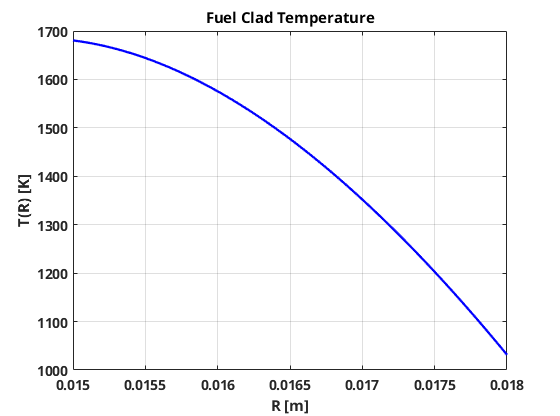
\includegraphics{lec30n-ex1-sol.png}
\caption{Cladding temperature profile.}
\label{fig:lec30n-ex1-sol}
\end{marginfigure}

\marginnote{

\vspace{0.25cm}

\noindent\textbf{Note:} Take a moment to think about this temperature profile and consider the following questions:
\begin{enumerate}

\item \textbf{Question:} What direction is heat flowing?  \textbf{Answer:} Heat is flowing from the cladding inner surface (inward heat flux is imposed as the boundary condition at the fuel/clad interface) through the cladding and out through the outer surface to the coolant. 
\item \textbf{Question:} Does the downward curvature of the temperature profile make sense?  \textbf{Answer:} Yes!  In heat transfer class you may have been taught that curvature of the temperature profile indicates heat generation in the region.  In this case, it is not \emph{heat generation} so much as it is \emph{heat deposition} but it acts the same mathematically.

\item \textbf{Question:} What controls the temperature at the inner and outer surface of the cladding? (there were no type 1 boundary conditions)  \textbf{Answer:} The outer surface temperature is related to: a) the amount of heat that must be passed through the boundary---all the heat passed into the cladding from the fuel plus all of the heat deposited in the cladding due to the radiation; and b) the coolant temperature, $T_{\infty}$, and convective heat transfer coefficient.
\end{enumerate}
}

\begin{lstlisting}[style=myMatlab,name=lec30n-ex1]
clear
clc
close 'all'

%% Parameters
R = 1.5e-2; % m, radius of fuel
w = 3.0e-3; % m, thickness of cladding
k = 16.75; % W/(m-K), thermal conductivity of clad
Q = 1e8; % W/m^2, Source term from heat dep in cladding.

Q2 = 6.32e5; % W/m^2, Heat flux due to heat produced in fuel.
T_inf = 423; % K, temperature of water flowing on cladding
h = 1e4; % W/(m^2-K), convective heat transfer coefficient

%% Encode the governing equation and boundary conditions

F = @(r,T) [T(2); -(1./r)*T(2) - Q./(k*r)*exp(-r/R)];
bcfun = @(Ta,Tb) [Ta(2)+ Q2/k; ...
    Tb(2) + (h/k)*(Tb(1)-T_inf)];

%% Establish initial mesh and solution estimate
rMin = R; rMax = R+w; nR = 200;
Tguess = [T_inf 0];
solinit = bvpinit(linspace(rMin,rMax,nR),Tguess);

%% Solve and plot the result
sol = bvp5c(F,bcfun,solinit);

figure(1)
plot(sol.x,sol.y(1,:),'-b','linewidth',2);
title('Fuel Clad Temperature','fontsize',16,...
    'fontweight','bold');
xlabel('R [m]','fontsize',14,'fontweight','bold');
ylabel('T(R) [K]','fontsize',14,'fontweight','bold');
grid on
set(gca,'fontsize',12,'fontweight','bold');
\end{lstlisting}

\newthought{Readers are encouraged} to read and consider the questions and answers posed in the margin.  Do not forget that \emph{the purpose of computing is insight.}  We are not solving these equations like they are a puzzle or to make impressive pictures but rather to improve our understanding of the physical processes represented by the boundary value problem.  Take some time to run the MATLAB example and then experiment by changing parameters such as the thermal conductivity of the cladding, $k$, the convective heat transfer coefficient, $h$, or the source term for heat deposition in the cladding, $Q$. Do the changes you see to the results make sense?  How can you, as an engineer, actually change those parameters in a real physical system?

\subsection{Example Problem \#2}

From the reactor fuel pin in Example \#1, consider the inhomogeneous source term representing heat deposition in the cladding material:
\begin{equation*}
S(r) = -10^8\frac{e^{-r/R}}{r}
\end{equation*}
Suppose that the leading constant of $10^8$ was an \emph{unknown parameter}, $Q$.  We might pose a question like: How high can $Q$ be while maintaining temperature at the cladding inner surface, $T(r=R)$, less than 1500K?  Clearly, all other parameters being the same, $Q$ would have to be \emph{smaller} than $10^8$ since, from our calculation in Example \#1, for that value the cladding inner surface temperature is nearly 1700K.  

We \emph{could} approach this problem by systematically changing $Q$ by hand and running the script.  MATLAB allows users to build \emph{parameters} into the boundary value problems that are being solved and determine these parameter values as part of the solution process.

\newthought{To use this} feature, we must take the following steps:
\begin{enumerate}
\item We include this parameter in our definition of the ODE function:
\begin{lstlisting}[style=myMatlab]
% add Q to my arguments for F
F = @(r,T,Q) [T(2); -(1./r)*T(2) - Q./(k*r)*exp(-r/R)];
\end{lstlisting}

\item The constraint on the parameter is added to the residual functions defined for the boundary conditions.

\marginnote{\textbf{Note:} Even though the function defined by \lstinline[style=myMatlab]{bcfun} does not make use of the third argument, $Q$, corresponding to the unknown parameter you must provide it as the third argument to our boundary condition function.

}
\begin{lstlisting}[style=myMatlab]
TgtTemp = 1500; % K
bcfun = @(Ta,Tb,Q) [Ta(2)+ Q2/k; ...
    Tb(2) + (h/k)*(Tb(1)-T_inf); ...
    Ta(1) - TgtTemp];
\end{lstlisting}

\item We also must supply an initial guess for the parameter when we initialize our solution.

\begin{lstlisting}[style=myMatlab]
rMin = R; rMax = R+w; nR = 200;
Tguess = [T_inf 0];
Qguess = 1e8;
solinit = bvpinit(linspace(rMin,rMax,nR),Tguess,Qguess);
\end{lstlisting}

\item The value for the parameter that meets our constraint is provided in the solution structure in the field named: \emph{parameters}.

\begin{lstlisting}[style=myMatlab]
sol2 = bvp5c(F,bcfun,solinit);
fprintf('Q = %g \n',sol2.parameters);
\end{lstlisting}

\end{enumerate}

The full script with these modifications is provided in the listing below. The resulting temperature profile is shown in Figure \ref{fig:lec30n-ex2-sol} and the $Q$ satisfying this constraint is: $Q = 8.361\times 10^{7}$. 

\begin{lstlisting}[style=myMatlab,name=lec30n-ex2]
R = 1.5e-2; % m, radius of fuel
w = 3.0e-3; % m, thickness of cladding
k = 16.75; % W/(m-K), thermal conductivity of clad
%Q = 1e8; % W/m^2, Source term from heat dep in cladding. 
Q2 = 6.32e5; % W/m^2, Heat flux due to heat produced in fuel.
T_inf = 423; % K, temperature of water flowing on cladding
h = 1e4; % W/(m^2-K), convective heat transfer coefficient

TgtTemp = 1500; % K

% add Q to my arguments for F
F = @(r,T,Q) [T(2); -(1./r)*T(2) - Q./(k*r)*exp(-r/R)];

% ... and for my BC functions
bcfun = @(Ta,Tb,Q) [Ta(2)+ Q2/k; ...
    Tb(2) + (h/k)*(Tb(1)-T_inf); ...
    Ta(1) - TgtTemp];
rMin = R; rMax = R+w; nR = 200;
Tguess = [T_inf 0];

% ... and add this to solinit
Qguess = 1e8;
solinit = bvpinit(linspace(rMin,rMax,nR),Tguess,Qguess);

sol2 = bvp5c(F,bcfun,solinit);

figure(2)
plot(sol2.x,sol2.y(1,:),'-b','linewidth',2);
title('Fuel Clad Temperature','fontsize',14,...
    'fontweight','bold');
xlabel('R [m]','fontsize',12,'fontweight','bold');
ylabel('T(R) [K]','fontsize',12,'fontweight','bold');
grid on
set(gca,'fontsize',10,'fontweight','bold');

fprintf('Q = %g \n',sol2.parameters);
\end{lstlisting}
\begin{marginfigure}[-12.0cm]
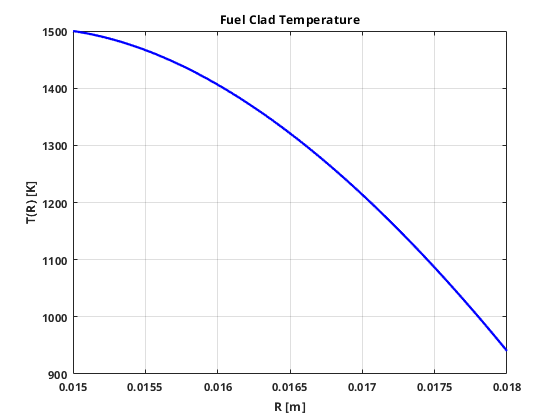
\includegraphics{lec30n-ex2-sol.png}
\caption{Temperature profile with constrained $Q$.}
\label{fig:lec30n-ex2-sol}
\end{marginfigure}
